%\VignetteIndexEntry{Sushi}
\documentclass{article}
\title{Sushi: An R/Bioconductor package for visualizing genomic data}
\author{Douglas H Phanstiel, Alan Boyle, Carlos Araya, and Mike Snyder}
\usepackage{Sweave}
\begin{document}
\Sconcordance{concordance:Sushi.tex:Sushi.Rnw:%
1 4 1 1 0 2 1 1 5 39 1 1 2 1 0 2 1 3 0 1 2 2 1 1 2 13 0 1 2 8 1 1 2 13 %
0 1 2 5 1 1 2 1 0 3 1 4 0 1 2 4 1 1 2 4 0 1 2 1 6 1 2 6 1 1 2 1 0 1 1 3 %
0 1 2 1 8 1 2 4 1 1 2 1 0 2 1 1 2 1 0 1 3 2 0 1 1 4 0 1 2 5 1 1 3 2 0 1 %
2 1 0 1 4 5 0 1 20 1 3 5 1 1 2 4 0 1 2 4 1 1 3 2 0 2 1 1 2 4 0 1 2 3 1 %
1 18 1 2 4 1 1 3 2 0 1 1 1 2 1 0 1 1 3 0 1 2 3 1 1 37 1 2 6 1 1 2 13 0 %
1 2 4 1 1 2 1 0 2 1 1 2 1 0 1 2 1 0 1 1 4 0 1 2 9 1 1 2 1 0 2 1 1 3 1 0 %
1 3 1 0 1 2 4 0 1 2 7 1 1 2 20 0 1 2 4 1 1 2 1 0 2 1 1 3 2 0 1 1 1 2 1 %
0 2 1 4 0 1 2 5 1 1 2 1 0 2 1 1 3 2 0 1 1 1 2 5 0 1 2 7 1 1 2 13 0 1 2 %
3 1 1 2 1 0 2 1 1 4 2 0 1 2 1 3 5 0 1 2 4 1 1 2 1 0 2 1 1 4 2 0 1 2 1 3 %
5 0 1 2 4 1 1 2 1 0 2 1 1 4 2 0 1 7 5 0 2 2 4 0 1 2 4 1 1 2 1 0 2 1 1 4 %
2 0 1 7 5 0 2 2 4 0 1 2 4 1 1 2 1 0 4 1 1 3 1 0 1 4 2 0 1 2 1 4 2 0 2 2 %
4 0 1 2 7 1 1 2 13 0 1 2 4 1 1 3 2 0 4 1 4 0 1 2 20 1 1 2 1 0 1 1 3 0 1 %
2 2 1 1 2 1 0 2 1 1 3 1 0 2 2 1 1 3 0 1 2 2 1 1 10 1 2 3 1 1 2 1 0 1 1 %
1 2 1 1 3 0 1 2 1 1 1 19 1 2 3 1 1 3 2 0 1 3 1 0 3 1 1 3 1 0 1 3 1 0 3 %
1 3 0 1 2 2 1 1 39 1 3 3 1}

\maketitle
\section{Introduction}

Sushi is an R package for plotting genomic data stored in multiple common genomic formats including bed, bedpe, bedgraph format. The flexible code allows for integration of the plots into multipanel figures that can include plots made by sushi, R basecode, or other R packages.  Sushi allows for simple flexible plotting of gene structures, transcript structures, sequencing tracks, ChIP seq peaks, chromatin interactions, GWAS results and other commen genomic data types.   


\section{Example datasets}
To illustrate how Sushi works, we have included several publicaly available data sets in the package Sushi. The data types include RNA-seq, ChIP-seq, ChIA-PET, and HiC data and can be loaded using the following commands

\begin{Schunk}
\begin{Sinput}
> library('Sushi')
> Sushi_data = data(package = 'Sushi')
> data(list = Sushi_data$results[,3]) 
\end{Sinput}
\end{Schunk}

\section{plotManhattan}

Manhattan plots can be plotted given SNPS and significance values in bed format.

\begin{Schunk}
\begin{Sinput}
> head(Sushi_GWAS.bed)
\end{Sinput}
\begin{Soutput}
  chr.hg18 pos.hg18 pos.hg18.1       rsid pval.GC.DBP V6
1     chr1  1695996    1695996  rs6603811    0.003110  .
2     chr1  1696020    1696020  rs7531583    0.000824  .
3     chr1  1698661    1698661 rs12044597    0.001280  .
4     chr1  1711339    1711339  rs2272908    0.001510  .
5     chr1  1712792    1712792  rs3737628    0.001490  .
6     chr1  1736016    1736016 rs12408690    0.004000  .
\end{Soutput}
\end{Schunk}

The 'plotManhattan' function is used to plot the data while the 'labelgenome' function is used to add the genome labels to the x-axis.

\begin{center}

\begin{Schunk}
\begin{Sinput}
> # make color palette
> # make the plot
> plotManhattan(bedfile=Sushi_GWAS.bed,pvalues=Sushi_GWAS.bed[,5],col=topo.colors,genome=Sushi_hg18_genome,cex=0.75)
> # add labels
> labelgenome(genome=Sushi_hg18_genome,side=1,scipen=20,n=4,scale="Mb",edgeblankfraction=0.20,line=.18,chromline=.5,scaleline=0.5)
> # add y-axis
> axis(side=2,las=2,tcl=.2)
> mtext("log10(P)",side=2,line=1.75,cex=.75,font=2)
\end{Sinput}
\end{Schunk}
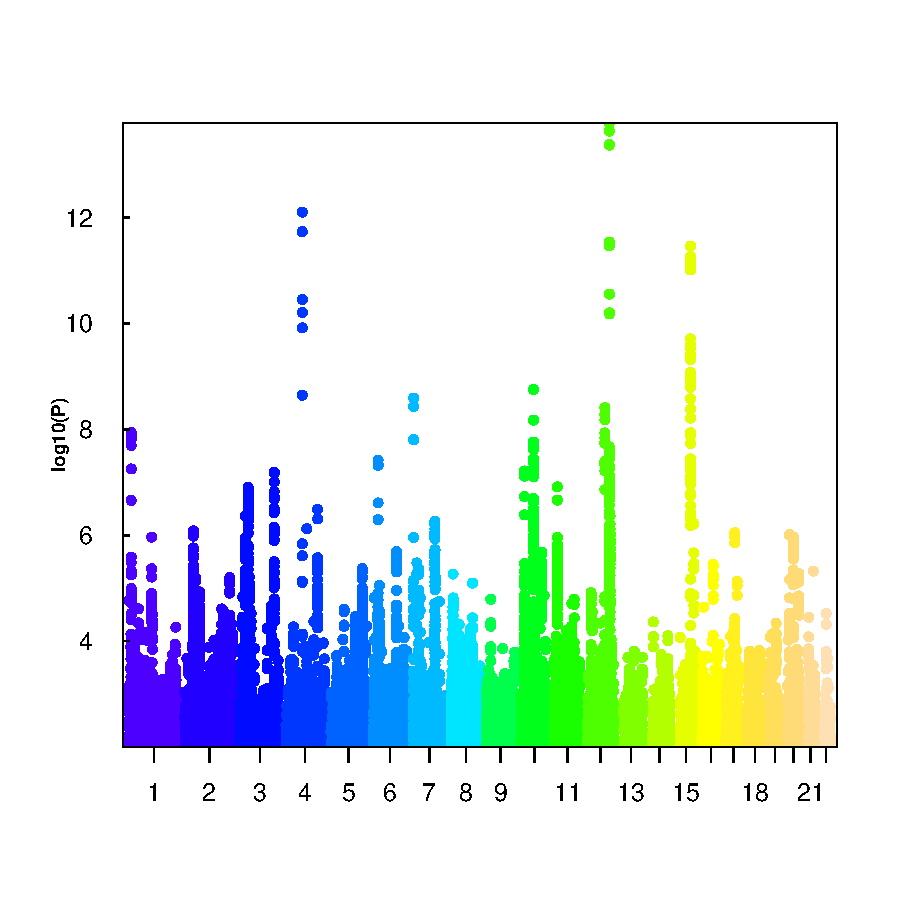
\includegraphics{Sushi-003}
\end{center}






\section{plotHiC}

HiC interactio plots can be plotted given an interaction matrix in which row and column names are genomic coordiates and matrix values are some tye of interaction score.

\begin{Schunk}
\begin{Sinput}
> Sushi_HiC.matrix[100:105,100:105]
\end{Sinput}
\begin{Soutput}
          3980000   4020000   4060000  4100000   4140000   4180000
3980000  0.000000 50.087965 49.689032 22.89760  7.438259  2.219527
4020000 50.087965 40.469337 33.922805 24.07214 12.652542  3.620466
4060000 49.689032 33.922805 26.998026 30.17873 21.879022  6.850893
4100000 22.897599 24.072145 30.178735 54.47335 48.570924 11.379299
4140000  7.438259 12.652542 21.879022 48.57092 45.265394 26.369969
4180000  2.219527  3.620466  6.850893 11.37930 26.369969 11.413106
\end{Soutput}
\end{Schunk}

The 'plotHiC' function is used to plot the data while the 'labelgenome' function is used to add the genome labels to the x-axis.  'plotHiC' returns an object indicating the color palette and data range that can be fed into 'addlegend' to create a legend.

\begin{center}

\begin{Schunk}
\begin{Sinput}
> # set the genomic regions
> chrom            = "chr11"
> chromstart       = 500000
> chromend         = 5050000
> # plot the HiC data
> phic = plotHic(Sushi_HiC.matrix,chrom,chromstart,chromend,max_y = 20,zrange=c(0,28),flip=FALSE)
> # add the legend
> addlegend(phic[[1]],palette=phic[[2]],title="score",side="right",bottominset=0.4,topinset=0,xoffset=-.035,labelside="left",width=0.025,title.offset=0.035)
> # add labels
> labelgenome(chrom,chromstart,chromend,side=1,scipen=20,n=4,scale="Mb",edgeblankfraction=0.20,line=.18,chromline=.5,scaleline=0.5)
> 
> 
\end{Sinput}
\end{Schunk}
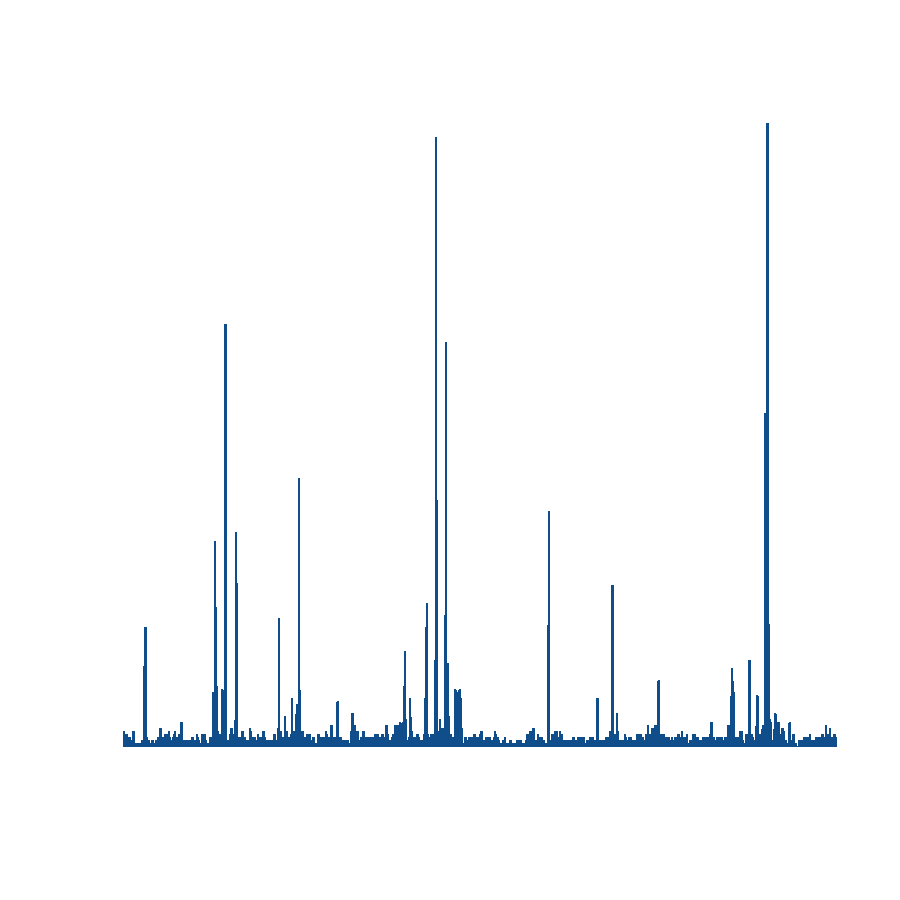
\includegraphics{Sushi-005}
\end{center}

plotHic has a number of customizable options.  The plot can be flipped over the x-axis by setting flip = TRUE.  The color palette can be changed by the palette argument. 

addlegend also has customizable features.  The legend can be moved to the left side of the plot by setting side = "left" and the labeling canbe moved to the right side of the lenged buy setting labelside = "right".  The vertical position of the legend can be adjusted by changing the topinset and bottominset.

Finally, the x-axis label can be moved to the top of the plot by setting side = 3 in the labelgenome function.

\begin{center}

\begin{Schunk}
\begin{Sinput}
> # set the genomic regions
> chrom            = "chr11"
> chromstart       = 500000
> chromend         = 5050000
> # plot the HiC data
> phic = plotHic(Sushi_HiC.matrix,chrom,chromstart,chromend,max_y = 20,zrange=c(0,28),flip=TRUE,palette=colorRampPalette(c("black","blue","#5900E5","#E5001B","orange","yellow","white")))
> # add the legend
> addlegend(phic[[1]],palette=phic[[2]],title="score",side="left",bottominset=0.1,topinset=0.5,xoffset=-.035,labelside="right",width=0.025,title.offset=0.035)
> # add labels
> labelgenome(chrom,chromstart,chromend,side=3,scipen=20,n=4,scale="Mb",edgeblankfraction=0.20,line=.18,chromline=.5,scaleline=0.5)
\end{Sinput}
\end{Schunk}
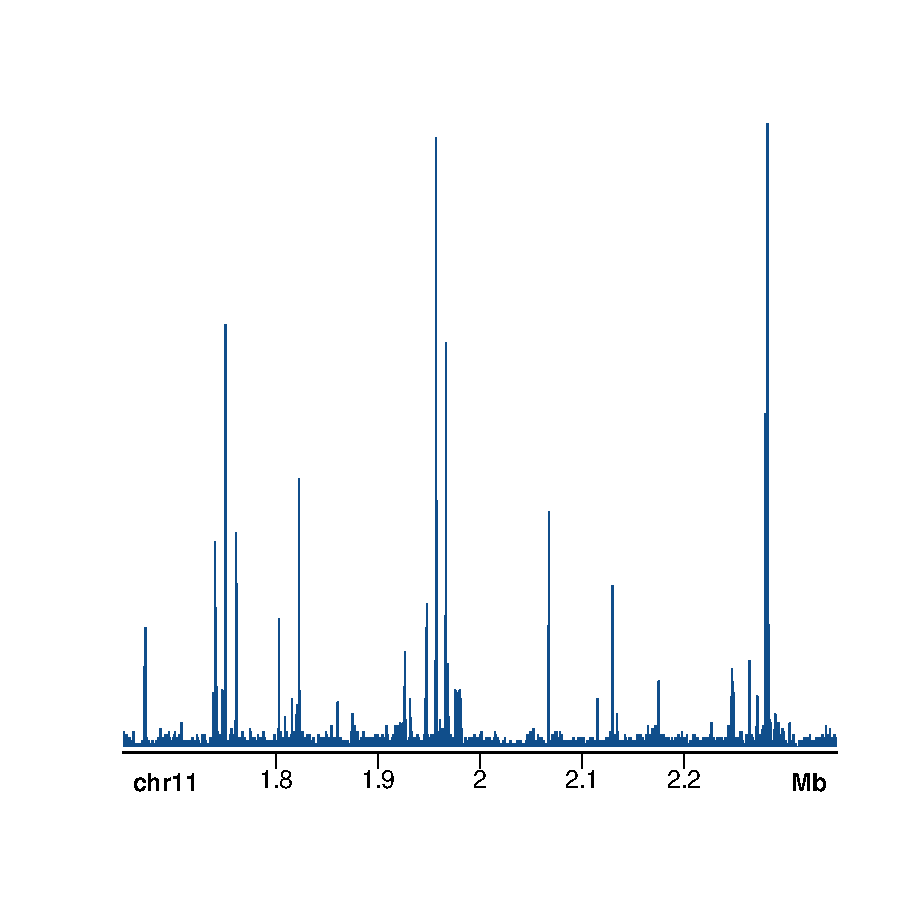
\includegraphics{Sushi-006}
\end{center}



\section{plotBedpe}

plotBedpe allows for data in bedpe format to be plotted in multiple fashions.  To illustrate this we will use 5C data formatted in the following way.

\begin{Schunk}
\begin{Sinput}
> head(Sushi_5C.bedpe)
\end{Sinput}
\begin{Soutput}
  chrom1    start1      end1 chrom2    start2      end2 name    score strand1
1   chr2 234208447 234223064   chr2 234156762 234159135   NA 44.39862       .
2  chr15  41711734  41718116  chr15  41802421  41808201   NA 20.62534       .
3  chr11  64172456  64183193  chr11  64068878  64079209   NA 16.91630       .
4   chr2 234208447 234223064   chr2 234163674 234170252   NA 12.34501       .
5   chr6  41755186  41769245   chr6  41435903  41452283   NA 11.63480       .
6  chr11  64159283  64172456  chr11  64068878  64079209   NA 11.13098       .
  strand2 samplenumber
1       .            1
2       .            1
3       .            1
4       .            1
5       .            1
6       .            1
\end{Soutput}
\end{Schunk}

plotBedpe can plot bedpe as arches.  The height, linewidth, and color of each arch can be scaled to represent different aspects of the data.  Here the height of the arches represents the Z-score of the 5C interaction, the color represents the cell line each interaction was detected in, and the line widths are kept constant.

\begin{center}

\begin{Schunk}
\begin{Sinput}
> # set the genomic regions
> chrom            = "chr11"
> chromstart       = 1650000
> chromend         = 2350000
> # plot the loops
> pbpe = plotbedpe(Sushi_5C.bedpe,chrom,chromstart,chromend,heights = Sushi_5C.bedpe$score,offset=0,
+                  flip=FALSE,bty='n',lwd=1,plottype="loops",colorby=Sushi_5C.bedpe$samplenumber,
+                  colorbycol=colorRampPalette(c("#5900E5","#E5001B","orange")))
> # add the genome labels
> labelgenome(chrom, chromstart,chromend,side=1,scipen=20,n=3,scale="Mb",line=.18,chromline=.5,scaleline=0.5)
> # add the legend
> legend("topright",inset =0.01,legend=c("K562","HeLa","GM12878"),col=c("#5900E5","#E5001B","orange"),pch=19,bty='n',text.font=2)
> # add y-axis
> axis(side=2,las=2,tcl=.2)
> mtext("Z-score",side=2,line=1.75,cex=.75,font=2)
\end{Sinput}
\end{Schunk}
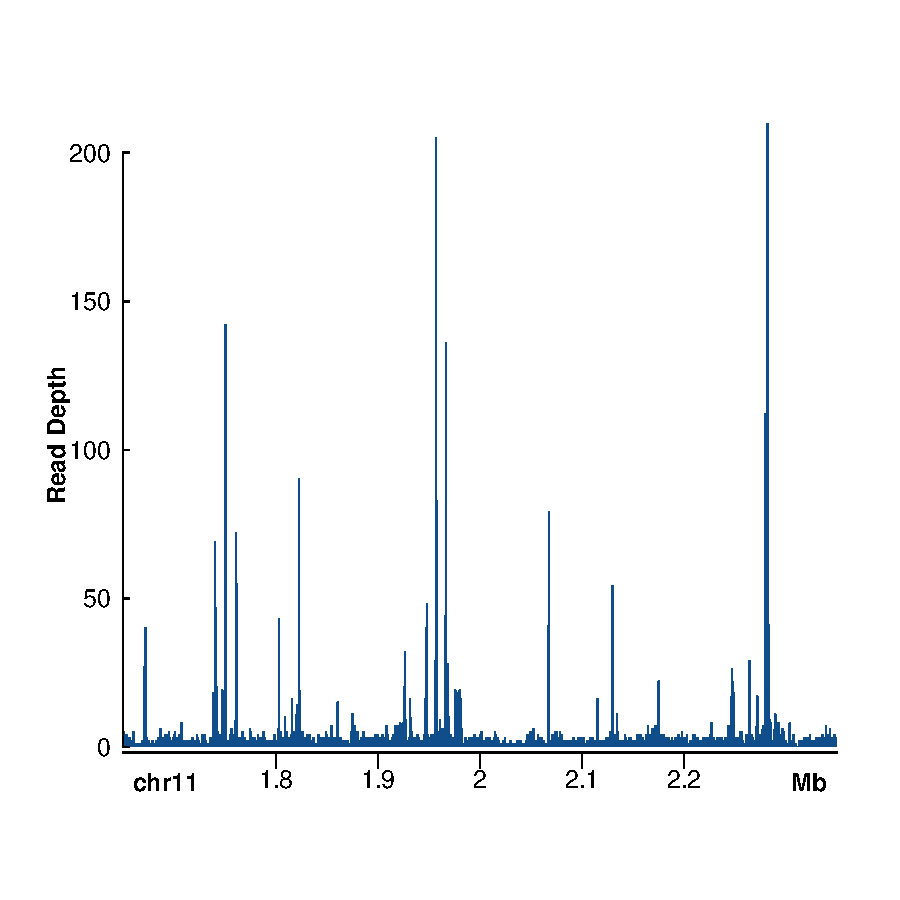
\includegraphics{Sushi-008}
\end{center}

The plot can be flipped over the x-axis by setting flip = TRUE,  Bedpe elements can be represented by boxes and straight lines by setting plottype = "lines".  And colors can be used to represent Z-scores by setting colorby = "Sushi_5C.bedpe$score". 

\begin{center}

\begin{Schunk}
\begin{Sinput}
> # set the genomic regions
> chrom            = "chr11"
> chromstart       = 1650000
> chromend         = 2350000
> # plot the lines
> pbpe = plotbedpe(Sushi_5C.bedpe,chrom,chromstart,chromend,offset=0,
+                  flip=TRUE,bty='n',lwd=1,plottype="lines",colorby=Sushi_5C.bedpe$score,
+                  colorbycol=colorRampPalette(c("black","blue","#5900E5","#E5001B","orange","yellow","white")))
> # add the genome labels
> labelgenome(chrom, chromstart,chromend,side=3,scipen=20,n=3,scale="Mb",line=.18,chromline=.5,scaleline=0.5)
> # add the legend
> addlegend(pbpe[[1]],palette=pbpe[[2]],title="Z-score",side="right",bottominset=0.05,topinset=0.05,xoffset=-.035,labelside="right",width=0.025,title.offset=0.035)
\end{Sinput}
\end{Schunk}
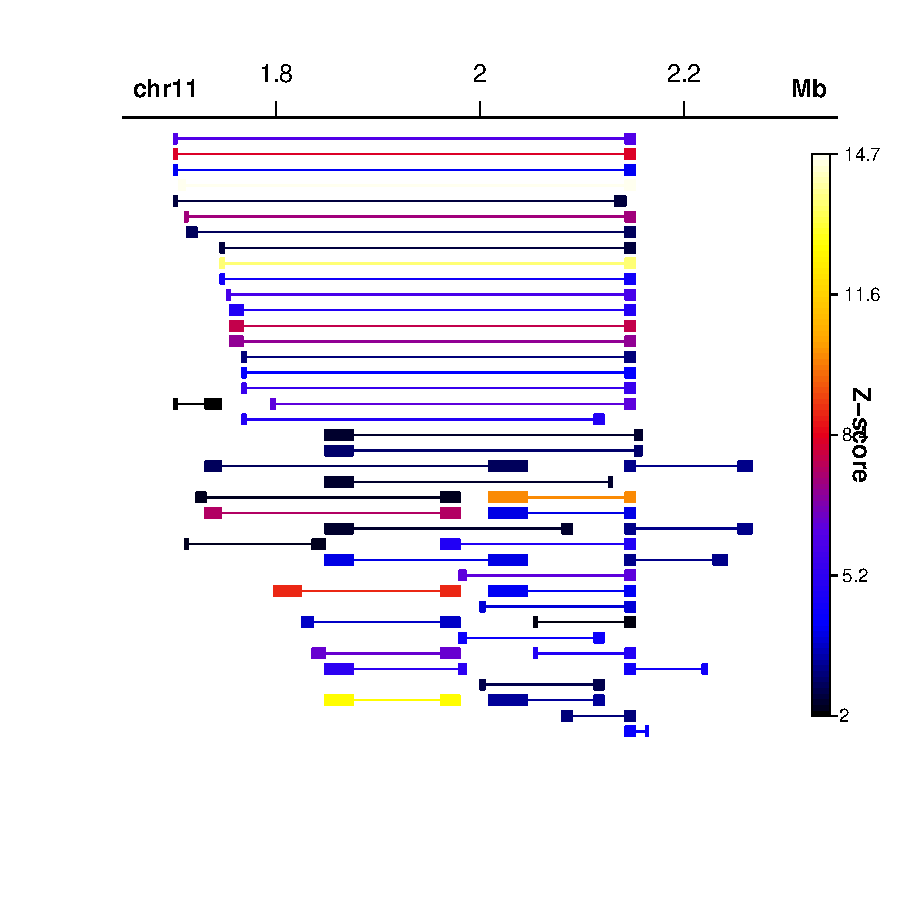
\includegraphics{Sushi-009}

\end{center}




\section{plotBedgraph}

Signal tracks can be plotted using the plotBedgraph.  The input requires data in bedgrpah format

\begin{Schunk}
\begin{Sinput}
> head(Sushi_DNaseI.bedgraph)
\end{Sinput}
\begin{Soutput}
  chrom start   end value
1 chr11 77224 77244     1
2 chr11 77244 77384     2
3 chr11 96704 96724     1
4 chr11 96724 96844     3
5 chr11 96844 96884     2
6 chr11 97904 97924     3
\end{Soutput}
\end{Schunk}

The 'plotBedgraph' function is used to plot the data while the 'labelgenome' function is used to add the genome labels to the x-axis.  The y-axis in added use basic R functions.

\begin{center}

\begin{Schunk}
\begin{Sinput}
> # set the genomic regions
> chrom            = "chr11"
> chromstart       = 1650000
> chromend         = 2350000
> # overlapping, transparent, and rescaled
> plotBedgraph(Sushi_DNaseI.bedgraph,chrom,chromstart,chromend,transparency=1.0,color="#5900E5",lwd=1,linecol="#5900E5")
> # add the genome labels
> labelgenome(chrom,chromstart,chromend,side=1,scipen=20,n=4,line=.18,chromline=.5,scaleline=0.5,scale="Mb")
> # add y-axis
> axis(side=2,las=2,tcl=.2)
> mtext("Read Depth",side=2,line=1.75,cex=1,font=2)
> 
\end{Sinput}
\end{Schunk}
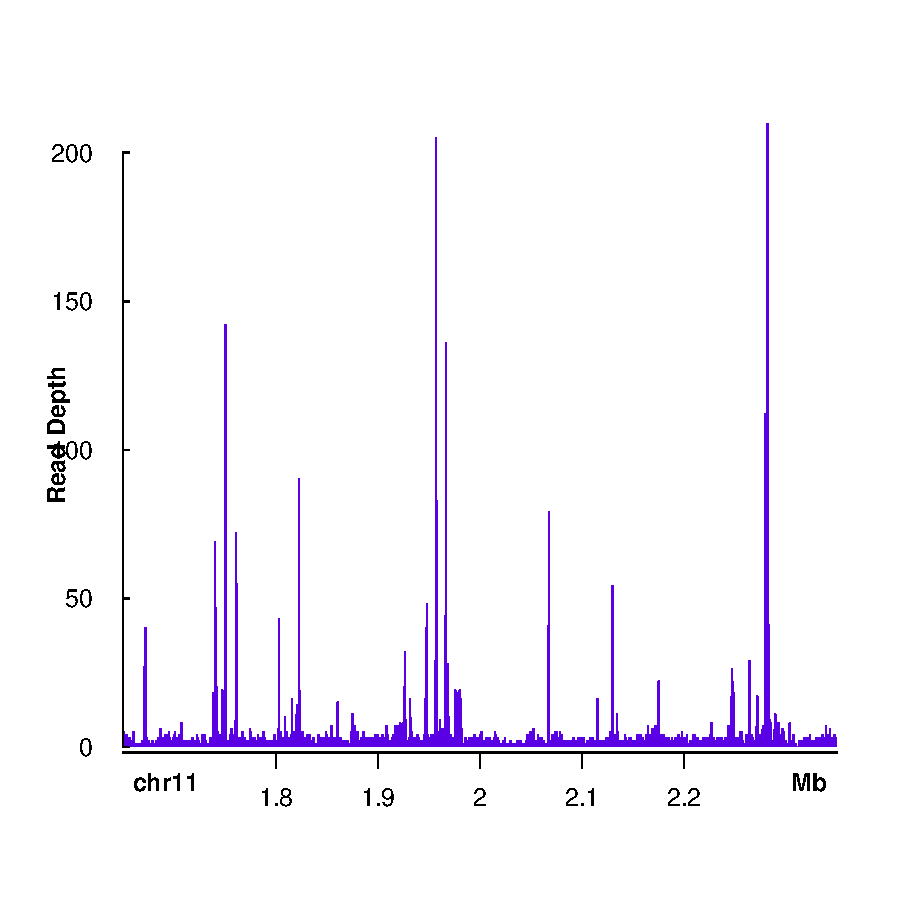
\includegraphics{Sushi-011}
\end{center}

Multiple bedgraph tracks can be plotted on the same plot by setting overlay=TRUE.  Transparencies can be added for easier viewing by adjusting the transcparency value.  The second plot can be rescaled to the maximum of the first plot by setting rescaleoverlay=TRUE.

\begin{center}
\begin{Schunk}
\begin{Sinput}
> # set the genomic regions
> chrom            = "chr11"
> chromstart       = 1955000
> chromend         = 1960000
> # plot chip-seq data
> plotBedgraph(Sushi_ChIPSeq_CTCF.bedgraph,chrom,chromstart,chromend,transparency=.50,flip=FALSE,color="blue",linecol="blue")
> # plot dnaseI data
> plotBedgraph(Sushi_DNaseI.bedgraph,chrom,chromstart,chromend,transparency=.50,flip=FALSE,color="#E5001B",linecol="#E5001B",overlay=TRUE,rescaleoverlay=TRUE)
> # add the genome labels
> labelgenome(chrom,chromstart,chromend,side=1,scipen=20,n=3,line=.18,chromline=.5,scaleline=0.5,scale="Kb")
> # set the legend colors
> transparency = 0.5
> col1 = col2rgb("blue")
> finalcolor1 = rgb(col1[1],col1[2],col1[3],alpha=transparency * 255,max = 255)
> col2 = col2rgb("#E5001B")
> finalcolor2 = rgb(col2[1],col2[2],col2[3],alpha=transparency * 255,max = 255)
> # add legend
> legend("topright",inset=0.025,legend=c("DnaseI","ChIP-seq (CTCF)"),fill=c(finalcolor1,finalcolor2),border=c("blue","#E5001B"),text.font=2,cex=1.0)
\end{Sinput}
\end{Schunk}
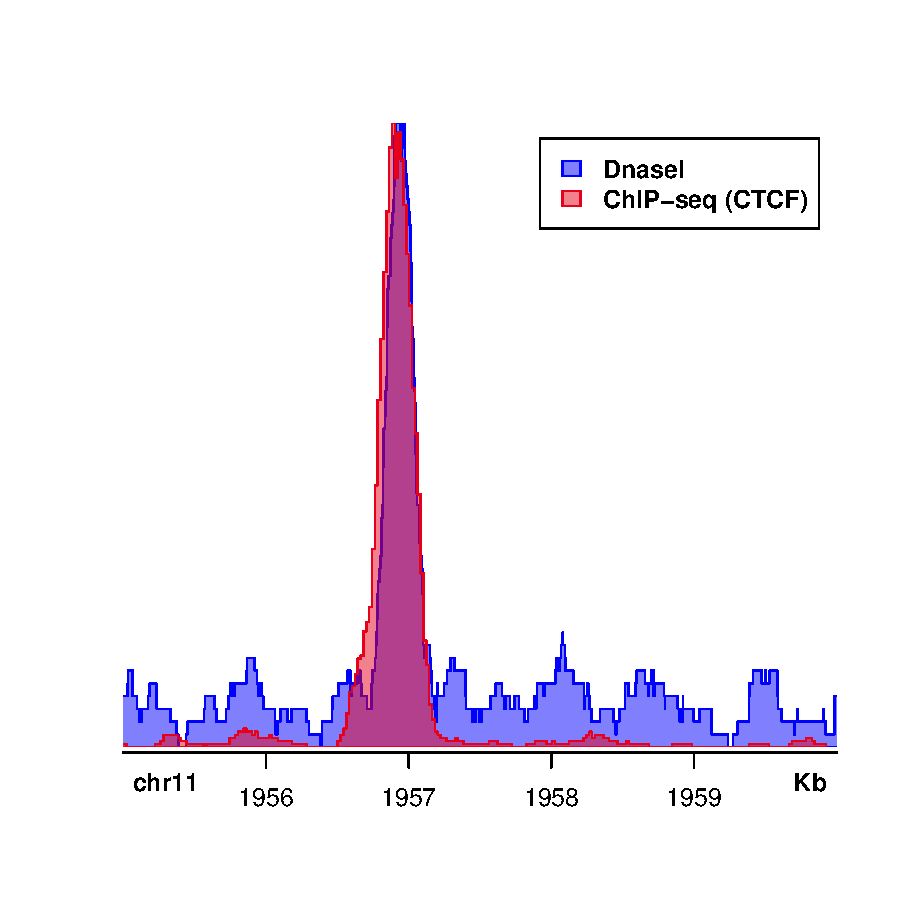
\includegraphics{Sushi-012}
\end{center}

Setting flip=TRUE is another method that can be used to compare tracks.


\begin{center}
\begin{Schunk}
\begin{Sinput}
> par(mfrow=c(2,1),mar=c(1,4,1,1))
> # set the genomic regions
> chrom            = "chr11"
> chromstart       = 1955000
> chromend         = 1960000
> # plot chip-seq data
> plotBedgraph(Sushi_ChIPSeq_CTCF.bedgraph,chrom,chromstart,chromend,transparency=.50,flip=FALSE,color="blue",linecol="blue")
> # add y-axis
> axis(side=2,las=2,tcl=.2)
> mtext("Read Depth",side=2,line=1.75,cex=1,font=2)
> # add legend
> legend("topright",inset=0.025,legend=c("DnaseI","ChIP-seq (CTCF)"),fill=c(finalcolor1,finalcolor2),border=c("blue","#E5001B"),text.font=2,cex=1.0)
> # plot dnaseI data
> plotBedgraph(Sushi_DNaseI.bedgraph,chrom,chromstart,chromend,transparency=.50,flip=TRUE,color="#E5001B",linecol="#E5001B",overlay=FALSE)
> # add y-axis
> ylabs = axis(side=2,las=2,tcl=.2,at=pretty(par("yaxp")[c(1,2)]),labels=-1*pretty(par("yaxp")[c(1,2)]))
> mtext("Read Depth",side=2,line=1.75,cex=1,font=2)
> # add the genome labels
> labelgenome(chrom,chromstart,chromend,side=3,scipen=20,n=3,line=.18,chromline=.5,scaleline=0.5,scale="Kb")
> # set the legend colors
> transparency = 0.5
> col1 = col2rgb("blue")
> finalcolor1 = rgb(col1[1],col1[2],col1[3],alpha=transparency * 255,max = 255)
> col2 = col2rgb("#E5001B")
> finalcolor2 = rgb(col2[1],col2[2],col2[3],alpha=transparency * 255,max = 255)
\end{Sinput}
\end{Schunk}
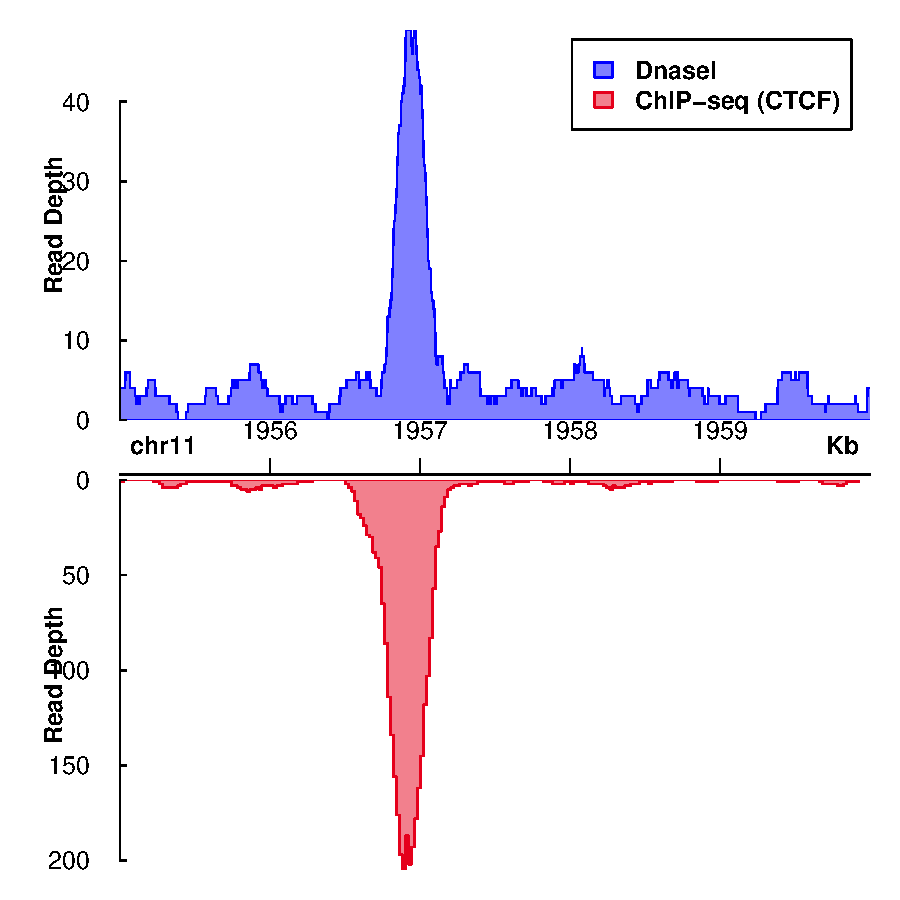
\includegraphics{Sushi-013}
\end{center}

\end{document}

?axis
